\documentclass{worksheetclass}

\usepackage{import}
\import{}{custom_macros.tex}

\title{Seiberg-Witten Theory}

% DOCUMENT -----------------------------

\begin{document}

\maketitle

\tableofcontents

\section{$\mN=2$ supersymmetric Yang-Mills theories}

    \subsection{Lagrangian}

        Let us start by considering a general SYM theory with gauge group $G$. The $\mN=2$ superfields for theories without gravities are the the hypermultiplet and the vector multiplet. The $\mN=2$ superspace being much more complicated, it is convenient to use use $\mN=1$ superspace and express the $\mN=2$ sueprfields in terms of $\mN=1$ superfields:
        \begin{align}
            [\mN=2 \text{ vector multiplet}] &: V=(\lambda_\alpha,A_\mu,D)\oplus \Phi=(\phi,\psi_\alpha,D)\\
            [\mN=2 \text{ hypermultiplet}] &: H_1=(H_1,\psi_{1\alpha},F_1)\oplus \bar{H}_2=(\bar{H}_2,\bar{\psi}_{2\dalpha},\bar{F}_2)
        \end{align}
        where $V$ is a vector superfield and $\Phi,H_1,H_2$ are chiral superfields. We use the notation
        \begin{align}
            \phi=\phi^a T_a,\quad \psi_\alpha=\psi^a_\alpha T_a,\quad F=F^a T_a,\\
            \lambda=\lambda^a T_a,\quad \D_\alpha=\D^a_\alpha T_a,\quad A_\mu=A^a_\mu T_a,
        \end{align}
        where $\{T_a\}_{a=1,\dots,\dim G}$ are the generators of $\mathfrak{g}$, the complexified Lie algebra of $G$. Note that all fields except $A_\mu$ are complex and therefore actually belong to the complexified Lie algebra $\mathfrak{g}_\C\equiv\C\otimes\mathfrak{g}=\mathfrak{g}+i\mathfrak{g}$.
        
        The representation under which the fields transform is dictated by their $\mN=2$ origin: $V$ and $\Phi$ must transform in the adjoint representation of the gauge group while $H_1$ and $\bar{H}_2$ buth transform in any representation $R$. Our notation implies that $H_2$ transform in the complex conjugate representation $\bar{R}$.

        The R-symmetry group is $\U(2)_R$ and the lagrangian should be invariant under its compact component $\SU(2)_R$. This is a necessary and sufficient condition to have $\mN=2$ supersymmetry. All bosonic fields $A_\mu,D,F$ and $\phi$ transform as singlets and $(\lambda_\alpha,\psi_\alpha)$ transform as a doublet.

        The most general pure gauge lagrangian reads
        \begin{eqnarray}
            \L^{\mN=2}_{\text{SYM}} = \frac{1}{32\pi}\Im\left[\tau\int\d^2\theta~W^\alpha W_\alpha\right] + \in\d^2\theta\d^2\bar{\theta}~\tr\left(\bar{\Phi}e^{2gV}\Phi\right)\label{eq:N2lag}
        \end{eqnarray}
        We note that the lagrangian does not have a superpotential. The auxiliary fields equation of motions are
        \begin{align}
            F^a &= 0,\\
            D^a &= -g[\phi,\phi^\dagger]^a.
        \end{align}
        Even though there is no superpotential, there is still a potential term of the scalar fields coming from the D-terms, it reads
        \begin{eqnarray}
            V(\phi,\phi^\dagger)=\frac{1}{2}D^aD_a=\frac{1}{2}g^2\tr[\phi,\phi^\dagger]^2.\label{eq:potential}
        \end{eqnarray}

    \subsection{Classical moduli space of vacua}

        The potential \eqref{eq:potential} vanishes if and only if $\phi$ belongs to the complexified Cartan $\mathfrak{h}_\C$ of $\mathfrak{g}$. At a general point of the moduli space, the scalar fields matrices can be diagonalized using the gauge symmetry. The moduli space is therefore parametrized by the eigenvalues of the matrices, i.e. by $r$ complex numbers, where $r$ is the rank the $\mathfrak{h}$. The diagonalization step does not fully breaks the gauge symmetry, there still is $U(1)^r$ symmetry. The low energy dynamic is the that of $r$ massless vector multiplets and $\dim G-r$ massive ones, with masses depending on the specific VEV's.

        Since there is only scalar fields coming from the vector superfield (transforming in the adjoint representation), there is only a Coulomb branch $\M_V$ and the Higgs branch $\M_H$ is empty. The classical moduli space is therefore
        \begin{eqnarray}
            \M_c = \M_{V,c}\times\M_{H,c}=\frac{\C^r}{W_G}\label{eq:classicalmodulispaceproduct}
        \end{eqnarray}
        where the $W_G$ factor is the Weyl group of the Cartan subalgebra, the remenant of the gauge symmetry that acts and the Cartan algebra.\todo{clarify with the $U(1)$'s}

        \begin{figure}[H]
            \centering
            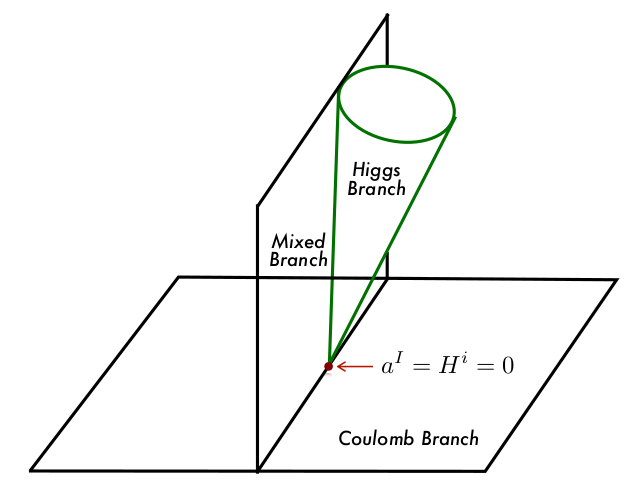
\includegraphics[scale=0.35]{Pictures/classicalmodulispace.png}
            \caption{$\mN=2$ classical moduli space, from \cite{bertolinisusy}.}
        \end{figure}

    \subsection{Quantum moduli space of vacua}

        We have seen the classical part of the story for the moduli space. How does quantum corrections change it? This a complicated question and it the goal of these notes to explain how to answer it. At this point, we can already anticipate three very important properties of the quantum moduli space $\M_q$:
        \begin{enumerate}
            \item \textbf{Product structure:} the $\mN=2$ selection rule that dictates that the classical moduli space has to look locally like a product \eqref{eq:classicalmodulispaceproduct} comes from the supersymmetry algebra and therefore also holds at the quantum level. Hence, locally, we have
            \begin{equation}
                \M_q = \M_{V,q}\times\M_{H,q}.\label{eq:quantummodulispaceproduct}
            \end{equation}
            \item \textbf{The Higgs branch is classically exact:} $\mN=2$ supersymmetry implies that the special Kähler metric on $\M_{V,c}$ and that the imaginary part if the generalized complexified gauge coupling $\tau_{IJ}$ are related. The former only depends on the scalar fields $\phi^I$ while the latter undergoes renormalization at one-loop. Its quantum-corrected expression is a function of the strong-coupling scale $\Lambda$, which therefore appears in the lagrangian in the same way as a VEV of a scalar belonging to a vector multiplet. However, the metric does not depend on those scalars and therefore doe snot depend on $\Lambda$ either. This means that taking the limit $\Lambda\to0$ will not change the metric in anyway; it classically exact:
            \begin{equation}
                \M_{H,c}=\M_{H,q}.
            \end{equation}
            On the other hand, the metric on the Coulomb brach can receive quantum corrections and solving the theory boils down to finding this metric. This explain why we will mostly focus on the Coulomb branch metric.
            \item \textbf{Existence of moduli space:} in $\mN=2$ theories, the moduli space can never be completely lifted, unlike for $\mN=1$ theories for example. This is obvious for the Higgs branch; since it is classicaly exact, existance at classical level implies existence at the quantum level. For the Coulomb branch on the other hand, it is less obvious and it is explained in \cite[p. 282]{bertolinisusy}.
        \end{enumerate}

        What about singularities? The classical moduli space admits singularities of enhanced gauge symmetry. However, the quantum moduli space cannot admit such singularities. This a result that we will show in the following. More precisely, it can have singularities where some massive particles become massless but those particles will never be gauge fields.There are no point of enhanced gauge symmetry and the theory is always in the Coulomb phase. In stead, there exist other types of singularities, such as Argyres-Douglas singularities for example, where mutually non-local particles become simultaneously massless.

        \begin{figure}[H]
            \centering
            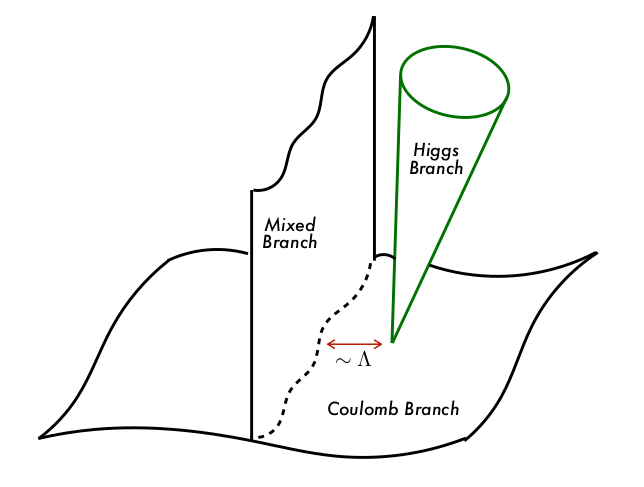
\includegraphics[scale=0.35]{Pictures/quantummodulispace.png}
            \caption{$\mN=2$ quantum moduli space, from \cite{bertolinisusy}.}
        \end{figure}

\section{Low energy effective actions}

    \subsection{General discussion}

        The leading dynamic of any (supersymmetric or non-supersymmetric) asyptotically free theory around a vacua where the potential vanishes is governed by massless fields. In this limit, the theory is scale invariant, by definition, and is at an IR fixed point of the RG flow. However, the nature of this IR fixed point can be if two kinds:
        \begin{enumerate}
            \item If no massless fields are present initially, there are no propagating degrees of freedom in the low-energy limit and the IR fiwed point is trivial.
            \item If the initial theory contains some massless fields, the theory can be in a free or interacting phase and the IR fixed point is non-trivial.
        \end{enumerate}
        
        \begin{theorem}[Colemann-Gross]
            In four spacetime dimensions, any theory of scalars, spinors and abelian gauge fields flows in the IR to a free (or trivial if everything gets a mass) theory.
        \end{theorem}
        This provides us with a necessary condition for having an interacting conformal field theory at low energy: there must be at least one massless non-abelian gauge field in the low-energy effective action. Note there are no general tool to study strongly coupled, interacting conformal field theories.

        Motivated by the previous discussion, we will only focus on effective theories that have scalars, spinors and abelian gauge fields. This is not such a restriction since for both $\mN=2$ and $\mN=4$ theories, a large fraction of the moduli space enjoys such an abelian, IR-free phase.
        
        What is the field content of the effective action ? A massless charged field will becomes massive though Higgs mechanism and then decouple as the energy scale is taken to be lower than the mass, so it cannot appear in the effective action. If, on the contrary, a massless is charged, it would still decouple and not appear in the effective action. We conclude that only massless neutral fields can appear in the low energy effective action. The low energy effective lagrangian must be of the form
        \begin{equation}
            \L = g_{ij}(\phi)\p\mu\phi^i\p^\mu\phi^j+\frac{1}{2}\Im[\tau_{IJ}(\phi)\F^I_{\mu\nu}\F^{J~\mu\nu}]+\text{ fermions}
        \end{equation}
        where $i,j$ run on neutral massless scalar fields and $I,J$ on abelian gauge fields. The \emph{complexified gauge coupling} $\tau_{IJ}$ and the field strength are defined as follows:
        \begin{equation}
            \tau_{IJ}=\frac{\theta_{IJ}}{2\pi}+\frac{4\pi i}{g^2_{IJ}}.
        \end{equation}
        The sigma-model metric $g_{ij}(\phi)$ is the metric on the moduli space $\M$, whose coordinates are the massless scalar fields VEV's.

    \subsection{$\mN=2$ effective action}

        Let us focus on $\mN=2$ supersymmetric theories and start from the most general asymptotically free renormalizable action. This action is fully characterized by the gauge group $G$ and the matter content, it is given by \eqref{eq:N2lag} for a pure gauge theory.

        It is known (just from supersymmetry) that the low energy effective lagrangian\footnote{By ``low energy effective lagrangian'', we mean the part of the effective lagrangian that contains the leading terms when the momenta vanish. In the full effective lagrangian there are of course infinitely many higher derivative terms. These are not governed by holomorphic quantities and we therefore have no control on them regarding quantum corrections.} must be of the for the form
        \begin{equation}
            \L^{\mN=2}_{\text{eff}} = \frac{1}{4\pi}\Im\left[\int\d^2\theta\d^2\bar{\theta}~K(\Phi,\bar{\Phi})+\int\d^2\theta\left(\frac{1}{2}\sum\tau(\Phi)W^\alpha W_\alpha\right)\right]
        \end{equation}
        with
        \begin{equation}
            K(\Phi,\bar{\Phi})=-\frac{i}{32\pi}\pdv{\F(\Phi)}{\Phi^a}\bar{\Phi}^a+\text{h.c.},\qquad \F_{ab}(\Phi)=\pdv{\F(\Phi)}{\Phi^a}{\Phi^b}.\label{eq:effectivelagftcs}
        \end{equation}
        It is therefore completely determined by the holomorphic function $\F$, called the \emph{prepotential}. The same model can be obtained from the usual lagrangian by just relaxing the renormalizability condition. We recover a renomalizable lagrangian by taking $\F(\Phi)=\frac{1}{2}\tau\tr\Phi^2$

        The map $K(A,\bar{A})$ is the Kähler potential, which gives a supersymmetric non-linear sigma-model for the field $\Phi$. It defines a metric on the moduli space as
        \begin{equation}
            ds^2=g_{i\bar{j}}(\Phi,\bar{\Phi})\d\Phi^a\d\bar{\Phi}^b = \pdv{K(\Phi,\bar{\Phi})}{\Phi^a}{\bar{\Phi}^b}\d\Phi^a\d\bar{\Phi}^b.
        \end{equation}
        From \eqref{eq:effectivelagftcs}, we see that 
        \begin{equation}
            ds^2=\pdv{K(\Phi,\bar{\Phi})}{\Phi^a}{\bar{\Phi}^b}\d\Phi^a\d\bar{\Phi}^b = \Im\left[\pdv{\F(\Phi)}{\Phi^a}{\Phi^b}\right]\d\Phi^a\d\bar{\Phi}^b
        \end{equation}
        thus the coefficients $\F_{ab}$ can be interpreted as coupling constant but they are also related to the metric on the moduli space.

        The potential is the effective lagrangian is given by
        \begin{equation}
            V(\phi,\phi^\dagger)=-\frac{1}{2\pi}\left(\Im\F_{ab}(\phi)\right)^{-1}[\phi^\dagger,\F_c(\phi)T_c]^a[\phi^\dagger,\F_d(\phi)T_d]^b.
        \end{equation}
        The Coulomb branch is therefore a Kähler manifold. Since the the Kähler potential can be written in terms of a holomorphic function as in \eqref{eq:effectivelagftcs}, it is more precisely a special Kähler manifold.

        If we were to add a hypermultiplet, we would have to additional complex scalars (one from each chiral superfields of the decomposition of the hypermultiplet). This new sigma-model would then define quaternionic manifold known as a Hyperkähler manifold. Due to the existence of those two sets of scalars (those belonging to the vector multiplet and those belonging to the hypermultiplet), the classical moduli space has the more general form
        \begin{equation}
            \M_c=\M_V\times\M_H
        \end{equation}
        where $\M_V$ is a Kähler manifold and $\M_H$ a Hyperkähler manifold.


    \section{$\SU(2)$ $\mN=2$ supersymmetric Yang-Mills theory in $D=4$}

    

\section{Generalization to other groups}

\section{SW geometry from string duality}



\printbibliography

\end{document}